\chapter{Design}

The goal is to create a C-like language which then compiles down to GPIR code.
The language should be as C-like as possible ideally we would like it to be as much
of a complete subset of C++ as possible, as the reset of the framework (Task Kernels and calling code)
are written in C++ and is more consistent with how the entire framework works.

C++ is a statically typed, imperative language which is sequentially evaluated by default.
GPIR is a dynamically typed functional language which is evaluated in parallel by default.
Both of these are pretty much complete opposite so the language design has to be one of that
is like C++ and can be mapped onto GPIR without too much trouble.

\section{Language Design Decisions}

\subsection{Parallel Evaluation}
        GPIR is parallel evaluated by default, with a "seq" function which
        evaluates the given arguments in parallel. Making GPC abide by equivalent rules of parallel
        evaluation by default with optional sequential makes the most sense, and gives the
        power to do stuff. 


\subsection{Purely Functional}

In the GPRM jumping to labels is an expensive operation, to avoid
this function calls will need to be inlined, and loops unrolled 
as much as possible. The execution path will also need to be known 
during compile time to achieve this. 

Another one of the major benefits of being able to compute the execution
path at runtime is that recursive functions can be more efficiently parralelised
by the compiler. We'll use a Mergesort example to illustrate this.

\begin{lstlisting}[style=myGPC]

//Use Sort class from Kernel
GPRM::Kernel::Sort MS;

int size = 8

void merge_sort(int *a, int low, int high) {
    if (low + 1 < high) {
        mid = (low + high) / 2;
   
        seq {
            par {
                merge_sort(a, low, mid);
                merge_sort(a, mid, high);
            }
            MS.merge(a, low, mid, high);            
        }
    
)

void GPC_merge_sort(int *a) {
    merge_sort(a, 0, size);
}

\end{lstlisting}

The merge kernel calls be be reduced down to a tree:

\begin{center}
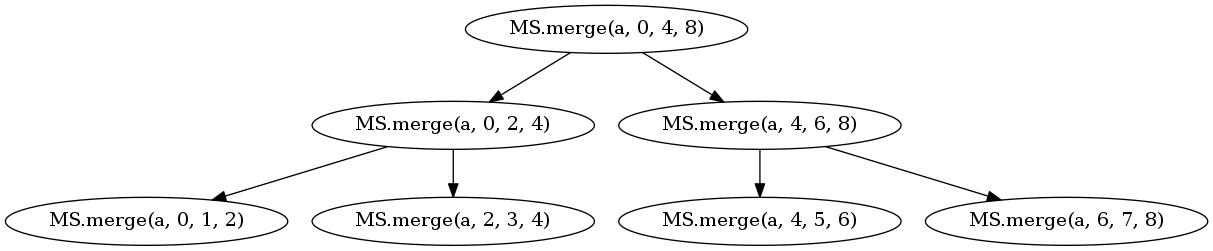
\includegraphics[scale=0.4]{graphs/mergesortTree.png}
\end{center}


\begin{lstlisting}[style=myGPC]

seq {

}

\end{lstlisting}

However if the language is Turing-complete deciding the execution path
of a given program is essentially the Halting Problem. It has been proven that the solution to this problem is undecidable\cite{halting} 

To avoid this problem, the language needs to be restricted to a point where it can still be useful and the execution
path decided at compile time.



   therefore
to avoid this the language itself will be purely functional.
        
        To allow for mapping tasks to different cores efficiently
        at compile time, the execution path must be able
        to be known at compile time. 
        
        For example given a tree-like
        recursion, 
        
        Single variable assignment
        and not allowing return values from kernel functions
        to be used in condition statements allow for this.

        To achieve this results from kernel functions are implicitly
        "tainted" as a kernel type.

        For example:
            int x = kernelObj.m1();
        has a return type of int.
        But the compiler implicitly casts this to a 
        kernel int.

        Kernel types can be passed to kernel methods, and even
        mixed with non kernel types when passed as arguments to
        kernel methods. For example:

        int y = 5;
        seq {
            int x = kernelObj.m1();
            kernelObj.m2(x + y);
        }

        would be allowed, but the following:

        int y = kernelObj.m1();



\section{Language Features}

    This section explains the features of the language with respect to the design decisions above.

\subsection{Syntax}
        The syntax aims to be as close to C/C++ as possible. Statements must end with a semicolon. 
        All variables must be statically typed. Blocks are surrounded in braces. Case is dependent.

\subsection{New Operators}
        Two new operators not currently present in C++ "seq" and "par" are introduced. 
        These are placed before a block
        of statements to determine whether each individual statement within the block are
        to be evaluated in sequential or parallel. By default a block of statements are evaluated
        in parallel, but the par keyword makes it more explicit especially if there's lots of nested
        seq/par blocks.

\subsection{Types}
        C++ types such as string, char, bool, int, and double are included.
        Pointers, and multi-level pointer types are included.
        However pointers are restricted in that you cannot take
        an address of any variable, adding and subtracting integers
        from pointers is allowed. Usually pointers are passed into
        the GPRM from the C++ caller to represent an Array.
        
\subsection{Operations}
        Most basic binary arithmetic operations are included i.e. 
        (+, -, *, /, \%, ==, !=, \&\&, ||, <<, >>, \&, |, \^) and
        unary operations :
        (-, ~, !) 
        are included. 

        (+=, ++, --, -=) are not included, due to the single assignment rule.
        Although an exception is made for the "afterthought" of the for loop construct, in which
        the integer loop variable can be incremented with += or decremented by -=.

\subsection{Functions}
        Exactly the same as C/C++ 


\subsection{Single assignment}
       Variables in GPC can only be assigned once per scope.

       for example the following wouldn't be allowed
           int i = 0;
           int i = i + 1;

       but the following would be:
           int i = 0;
           {
               int i = i;
           }

\subsection{For-Loops}
       For loops have the same syntax as C/C++ for loops with some restrictions.
       Essentially these are unrolled at compile-time and every iteration is evaluated in parallel.
       
       Essentialy the syntax is for(int var = n; [Boolean expression]; var += n or var -= n) 
